% Modified based on Xiaoming Sun's template
\documentclass{article}
\usepackage{amsmath,amsfonts,amsthm,amssymb}
\usepackage{setspace}
\usepackage{fancyhdr}
\usepackage{lastpage}
\usepackage{extramarks}
\usepackage{chngpage}
\usepackage{soul,color}
\usepackage{graphicx,float,wrapfig}
\usepackage{enumitem}
\usepackage{array} 
\usepackage{hyperref}
\usepackage{float}
\usepackage{fontspec}
\setmonofont{Consolas}
\usepackage{listings}
\usepackage{xcolor}

% \lstset{
%   basicstyle=\ttfamily
%   columns=fixed,       
%   numbers=left,                                        % 在左侧显示行号
%   numberstyle=\tiny\color{gray},                       % 设定行号格式
%   frame=none,                                          % 不显示背景边框
%   backgroundcolor=\color[RGB]{245,245,244},            % 设定背景颜色
%   keywordstyle=\color[RGB]{40,40,255},                 % 设定关键字颜色
%   numberstyle=\footnotesize\color{darkgray},           
%   commentstyle=\it\color[RGB]{0,96,96},                % 设置代码注释的格式
%   stringstyle=\rmfamily\slshape\color[RGB]{128,0,0},   % 设置字符串格式
%   showstringspaces=false,                              % 不显示字符串中的空格
%   language=c++,                                        % 设置语言
% }
\lstset{
  language = python, numbers=left, 
         numberstyle=\tiny,keywordstyle=\color{blue!70},
         commentstyle=\color{red!50!green!50!blue!50},frame=shadowbox,
         rulesepcolor=\color{red!20!green!20!blue!20},basicstyle=\ttfamily
}



\newcommand{\Class}{Pattern Recognition and Machine Learning}

% Homework Specific Information. Change it to your own
\newcommand{\Title}{Homework 6}

% In case you need to adjust margins:
\topmargin=-0.45in      %
\evensidemargin=0in     %
\oddsidemargin=0in      %
\textwidth=6.5in        %
\textheight=9.0in       %
\headsep=0.25in         %

% Setup the header and footer
\pagestyle{fancy}                                                       %
\chead{\Title}  %
\rhead{\firstxmark}                                                     %
\lfoot{\lastxmark}                                                      %
\cfoot{}                                                                %
\rfoot{Page\ \thepage\ of\ \protect\pageref{LastPage}}                          %
\renewcommand\headrulewidth{0.4pt}                                      %
\renewcommand\footrulewidth{0.4pt}                                      %

%%%%%%%%%%%%%%%%%%%%%%%%%%%%%%%%%%%%%%%%%%%%%%%%%%%%%%%%%%%%%
% Some tools
\newcommand{\enterProblemHeader}[1]{\nobreak\extramarks{#1}{#1 continued on next page\ldots}\nobreak%
                                    \nobreak\extramarks{#1 (continued)}{#1 continued on next page\ldots}\nobreak}%
\newcommand{\exitProblemHeader}[1]{\nobreak\extramarks{#1 (continued)}{#1 continued on next page\ldots}\nobreak%
                                   \nobreak\extramarks{#1}{}\nobreak}%

\newcommand{\homeworkProblemName}{}%
\newcounter{homeworkProblemCounter}%
\newenvironment{homeworkProblem}[1][Problem \arabic{homeworkProblemCounter}]%
  {\stepcounter{homeworkProblemCounter}%
   \renewcommand{\homeworkProblemName}{#1}%
   \section*{\homeworkProblemName}%
   \enterProblemHeader{\homeworkProblemName}}%
  {\exitProblemHeader{\homeworkProblemName}}%

\newcommand{\homeworkSectionName}{}%
\newlength{\homeworkSectionLabelLength}{}%
\newenvironment{homeworkSection}[1]%
  {% We put this space here to make sure we're not connected to the above.

   \renewcommand{\homeworkSectionName}{#1}%
   \settowidth{\homeworkSectionLabelLength}{\homeworkSectionName}%
   \addtolength{\homeworkSectionLabelLength}{0.25in}%
   \changetext{}{-\homeworkSectionLabelLength}{}{}{}%
   \subsection*{\homeworkSectionName}%
   \enterProblemHeader{\homeworkProblemName\ [\homeworkSectionName]}}%
  {\enterProblemHeader{\homeworkProblemName}%

   % We put the blank space above in order to make sure this margin
   % change doesn't happen too soon.
   \changetext{}{+\homeworkSectionLabelLength}{}{}{}}%

\newcommand{\Answer}{\ \\\textbf{Answer:} }
\newcommand{\Acknowledgement}[1]{\ \\{\bf Acknowledgement:} #1}

%%%%%%%%%%%%%%%%%%%%%%%%%%%%%%%%%%%%%%%%%%%%%%%%%%%%%%%%%%%%%


%%%%%%%%%%%%%%%%%%%%%%%%%%%%%%%%%%%%%%%%%%%%%%%%%%%%%%%%%%%%%
% Make title
\title{\textmd{\bf \Class: \Title}}
  \date{\textbf{\today}}
\author{\textbf{Qingru Hu \quad 2020012996}}
%%%%%%%%%%%%%%%%%%%%%%%%%%%%%%%%%%%%%%%%%%%%%%%%%%%%%%%%%%%%%

\begin{document}
\begin{spacing}{1.1}
\maketitle \thispagestyle{empty}

%%%%%%%%%%%%%%%%%%%%%%%%%%%%%%%%%%%%%%%%%%%%%%%%%%%%%%%%%%%%%
% Begin edit from here

\begin{homeworkProblem}
% \Answer \\
I use \href{https://hmmlearn.readthedocs.io/en/latest/}{\texttt{hmmlearn}} module to build HMM models.
\section*{(1)}
I use the \texttt{CategoricalHMM} model in \texttt{hmmlearn} to train the dataset, and 
I obtain from fitting the initial , the transition and emission probabilities, shown respectively 
in , Fig.2 and Fig.3.
\begin{table}[htbp]
  \centering
  \begin{tabular}{|c|c|c|}
    \hline
    Dice Type & Dice 1 & Dice 2 \\
    \hline 
    Initial Prob & 0.618 & 0.382 \\
    \hline
  \end{tabular}
  \caption{The initial probabilities}
\end{table}

\begin{table}[htbp]
  \centering
  \begin{tabular}{|c|c|c|}
    \hline
    Dice Type & Dice 1 & Dice 2 \\
    \hline 
    Dice 1 & 0.888 & 0.112 \\
    \hline
    Dice 2 & 0.156 & 0.844 \\
    \hline
  \end{tabular}
  \caption{The transition probabilities}
\end{table}

\begin{table}[htbp]
  \centering
  \begin{tabular}{|c|c|c|c|c|c|c|}
    \hline
    Dice/Point & 1 & 2 & 3& 4 & 5 & 6 \\
    \hline 
    Dice 1 & 0.158 & 0.164 & 0.184 & 0.171 & 0.191 & 0.132 \\
    \hline
    Dice 2 & 0.120 & 0.098 & 0.096 & 0.108 & 0.088 & 0.491 \\
    \hline
  \end{tabular}
  \caption{The emission probabilities}
\end{table}

The code is shown as below.
\begin{lstlisting}
import numpy as np
from hmmlearn import hmm

data = np.load('sequences.npy')
X = data.reshape(200*30, 1)
lens = np.ones(data.shape[0])*30
lens = lens.astype(int)
model = hmm.CategoricalHMM(n_components=2, random_state=10)
model.fit(X, lens)
model.score(X)
# -10434.902086730863
\end{lstlisting}

\section*{(2)}
\subsection*{Forward Algorithm}
The probability of observing sequence 6 6
6 6 using forward algorithm is $p = 0.015$.
\begin{lstlisting}
  iprob = model.startprob_
  tprob = model.transmat_
  eprob = model.emissionprob_
  
  for t in range(4):
      if t==0:
          a0 = eprob[0, 6]*iprob[0]
          a1 = eprob[1, 6]*iprob[1]
      else:
          a0 = eprob[0, 6]*(a0*tprob[0, 0] + a1*tprob[1, 0])
          a1 = eprob[1, 6]*(a0*tprob[0, 1] + a1*tprob[1, 1])
  p = a0 + a1
  # p = 0.014626307201743518
  \end{lstlisting}

\subsection*{Backward Algorithm}
The probability of observing sequence 6 6
6 6 using backward algorithm is $p = 0.015$.
\begin{lstlisting}
  iprob = model.startprob_
tprob = model.transmat_
eprob = model.emissionprob_

for t in [3, 2, 1, 0]:
    # as = np.zeros([2, 2])
    if t==3:
        b0 = 1
        b1 = 1
    else:
        b0 = tprob[0, 0]*eprob[0, 6]*b0 + tprob[0, 1]*eprob[1, 6]*b1
        b1 = tprob[1, 0]*eprob[0, 6]*b0 + tprob[1, 1]*eprob[1, 6]*b1
p = a0 + a1
# p = 0.014626307201743518
\end{lstlisting}

\section*{(3)}
This player is cheating and he switched his dice on his 12th roll.

\begin{lstlisting}
seq = np.array([3, 2, 1, 3, 4, 5, 6, 3, 1, 4, 1, 6, 6, 2, 6])
seq = seq.reshape(1, -1)
model.decode(seq)
# log_prob = -28.45720629383466,
# state_sequence = [0, 0, 0, 0, 0, 0, 0, 0, 0, 0, 0, 1, 1, 1, 1]
\end{lstlisting}

\end{homeworkProblem}

\begin{homeworkProblem}
In this problem, the datasets `iris', `breast\_cancer' and `usps' 
are represented as I, B and U. I select hyperparameter configuration that has the largest average
validation accuracy as the optimal for each model.
\section*{2.1}
\begin{lstlisting}
  models = {
    "Decision Tree": DecisionTreeClassifier,  # criterion, max_depth
    "Random Forest": RandomForestClassifier, # criterion, n_estimators
    "Bagging": BaggingClassifier, # n_estimators
    "Gradient Boosting": GradientBoostingClassifier, 
    # n_estimators, learning_rate
    # "XGBoost":
    "Naive Bayes": GaussianNB, # var_smoothing
    "Perceptron": Perceptron, # penalty, alpha
    "Logistic Regression": LogisticRegression, # penalty, C
    "LDA": LinearDiscriminantAnalysis,
    "SVM": SVC, # kernel, C
}
\end{lstlisting}

\section*{2.2}
\begin{lstlisting}
  model_hparams_best = {
    "Decision Tree": dict(criterion='gini', max_depth=5),
    "Random Forest": dict(n_estimators=50, criterion='entropy'),
    "Bagging": dict(n_estimators=20),
    "Gradient Boosting": dict(learning_rate=0.1, n_estimators=100),
    # "XGBoost":
    "Naive Bayes":dict(var_smoothing=1e-9),
    "Perceptron":dict(alpha=0.001, penalty='l1'),
    "Logistic Regression": dict(C=1, penalty='l2'),
    "LDA":dict(),
    "SVM":dict(kernel='rbf', C=1)
}
\end{lstlisting}

\section*{2.3}
\subsection*{Decision Tree}
\begin{table}[htbp]
  \centering
  \begin{tabular}{|c|c|c|c|c|c|c|c|c|c|}
  \hline
  criterion  & entropy & entropy & entropy & gini & gini & gini & log\_loss & log\_loss & log\_loss \\ \hline
  max\_depth & I    & B     & U      & I    & B     & U      & I    & B    & U \\ \hline
  3 & 0.933 & 0.895 & 0.923 & 0.933 & 0.895 & 0.944 & 0.933 & 0.912 & 0.937 \\ \hline
  5 & 0.933 & 0.912 & 0.909 & 0.933 & 0.947 & 0.923 & 0.933 & 0.912 & 0.93 \\ \hline
  10 & 0.933 & 0.912 & 0.923 & 0.933 & 0.912 & 0.937 & 0.933 & 0.912 & 0.93 \\ \hline
  12 & 0.933 & 0.895 & 0.944 & 0.933 & 0.912 & 0.937 & 0.933 & 0.912 & 0.937 \\ \hline
\end{tabular}
\end{table}
The best configuration of hyperparameters is \texttt{criterion='gini'} and \texttt{max\_depth=5}.

\subsection*{Random Forest}
\begin{table}[htbp]
  \centering
  \begin{tabular}{|c|c|c|c|c|c|c|c|c|c|}
  \hline
  criterion  & entropy & entropy & entropy & gini & gini & gini & log\_loss & log\_loss & log\_loss \\ \hline
  n\_estimators & I    & B     & U      & I    & B     & U      & I    & B    & U \\ \hline
  20 & 1.0 & 0.93 & 0.972 & 1.0 & 0.947 & 0.986 & 0.933 & 0.912 & 0.972 \\ \hline
  50 & 1.0 & 0.877 & 0.965 & 1.0 & 0.877 & 0.979 & 0.933 & 0.877 & 0.979 \\ \hline
  100 & 1.0 & 0.93 & 0.965 & 0.933 & 0.912 & 0.972 & 0.933 & 0.912 & 0.972 \\ \hline
  200 & 1.0 & 0.947 & 0.986 & 0.933 & 0.912 & 0.972 & 0.933 & 0.912 & 0.979 \\ \hline
\end{tabular}
\end{table}
The best configuration of hyperparameters is \texttt{criterion='entropy'} and \texttt{n\_estimators=50}.

\subsection*{Bagging}
\begin{table}[htbp]
  \centering
  \begin{tabular}{|c|c|c|c|}
  \hline
  n\_estimators/dataset & I    & B     & U \\ \hline
  2 & 0.867 & 0.982 & 0.951 \\ \hline
  5 & 0.867 & 1.0 & 0.944 \\ \hline
  10 & 0.933 & 1.0 & 0.951 \\ \hline
  20 & 0.933 & 0.982 & 0.986 \\ \hline
\end{tabular}
\end{table}
The best configuration of hyperparameters is \texttt{n\_estimators=20}.

\subsection*{Gradient Boosting}
\begin{table}[htbp]
  \centering
  \begin{tabular}{|c|c|c|c|c|c|c|c|c|c|}
  \hline
  learning\_rate  & 1e-3 & 1e-3 & 1e-3 & 1e-2 & 1e-2 & 1e-2 & 1e-1 & 1e-1 & 1e-1 \\ \hline
  n\_estimators & I    & B     & U      & I    & B     & U      & I    & B    & U \\ \hline
  10 & 1.0 & 0.632 & 0.909 & 0.933 & 0.632 & 0.909 & 1.0 & 0.632 & 0.93 \\ \hline
  20 & 0.933 & 0.632 & 0.93 & 0.933 & 0.632 & 0.909 & 0.933 & 0.965 & 0.909 \\ \hline
  50 & 0.933 & 0.947 & 0.937 & 0.933 & 0.965 & 0.923 & 1.0 & 0.947 & 0.951 \\ \hline
  100 & 0.933 & 0.632 & 0.909 & 1.0 & 0.632 & 0.93 & 1.0 & 0.632 & 0.93 \\ \hline
  200 & 0.933 & 0.632 & 0.909 & 0.933 & 0.965 & 0.909 & 1.0 & 0.965 & 0.937 \\ \hline
\end{tabular}
\end{table}
The best configuration of hyperparameters is \texttt{learning\_rate=0.1} and \texttt{n\_estimators=100}.

\subsection*{Naive Bayes}
\begin{table}[H]
  \centering
  \begin{tabular}{|c|c|c|c|}
  \hline
  var\_smoothing/dataset & I    & B     & U \\ \hline
  1e-09 & 1.0 & 0.982 & 0.93 \\ \hline
  1e-07 & 1.0 & 0.982 & 0.93 \\ \hline
  0.001 & 1.0 & 0.982 & 0.93 \\ \hline
  0.1 & 1.0 & 0.965 & 0.937 \\ \hline
\end{tabular}
\end{table}
The best configuration of hyperparameters is \texttt{var\_smoothing=1e-9}.

\subsection*{Perceptron}
\begin{table}[H]
  \centering
  \begin{tabular}{|c|c|c|c|c|c|c|c|c|c|}
  \hline
  penalty  & 1e-3 & 1e-3 & 1e-3 & 1e-2 & 1e-2 & 1e-2 & 1e-1 & 1e-1 & 1e-1 \\ \hline
  alpha & I    & B     & U      & I    & B     & U      & I    & B    & U \\ \hline
  1e-05 & 0.867 & 0.965 & 0.993 & 0.867 & 0.965 & 0.993 & 0.867 & 0.965 & 0.993 \\ \hline
  0.0001 & 0.867 & 0.947 & 0.993 & 0.867 & 0.912 & 0.986 & 0.867 & 0.982 & 0.986 \\ \hline
  0.001 & 0.867 & 0.947 & 0.993 & 0.867 & 0.965 & 0.986 & 0.867 & 0.947 & 0.937 \\ \hline
  0.01 & 0.867 & 0.965 & 0.993 & 0.867 & 0.965 & 0.993 & 0.867 & 0.965 & 0.993 \\ \hline
  0.1 & 0.867 & 0.912 & 0.986 & 0.867 & 0.982 & 0.986 & 0.8 & 0.93 & 0.937 \\ \hline
\end{tabular}
\end{table}
The best configuration of hyperparameters is \texttt{alpha=0.001} and \texttt{penalty='l1'}.

\subsection*{Logistic Regression}
The model solver `lbfgs' can not handle `l1' penalty, so I just include `None' and `l2' in penalty options.
\begin{table}[H]
  \centering
  \begin{tabular}{|c|c|c|c|c|c|c|}
  \hline
  penalty  & None & None & None & l2 & l2 & l2 \\ \hline
  C & I    & B     & U      & I    & B     & U    \\ \hline
  0.1 & 1.0 & 0.982 & 0.965 & 1.0 & 0.982 & 0.986 \\ \hline
  1 & 0.867 & 0.982 & 0.986 & 1.0 & 0.982 & 0.965 \\ \hline
  10 & 1.0 & 0.982 & 0.965 & 1.0 & 0.982 & 0.979 \\ \hline
\end{tabular}
\end{table}
The best configuration of hyperparameters is \texttt{C=1} and \texttt{penalty='l2'}.

\subsection*{LDA}
\begin{table}[H]
  \centering
  \begin{tabular}{|c|c|c|c|}
  \hline
  dataset & I    & B     & U \\ \hline
  validation accuracy & 1.0 & 0.930 & 0.993 \\ \hline
\end{tabular}
\end{table}
The average of the validation accuracy over the three datasets is $0.978$.

\subsection*{SVM}
\begin{table}[H]
  \centering
  \begin{tabular}{|c|c|c|c|c|c|c|c|c|c|c|c|c|}
  \hline
  kernel  & linear & linear & linear & poly & poly & poly & rbf & rbf & rbf &sigmoid &sigmoid &sigmoid  \\ \hline
  C & I    & B     & U      & I    & B     & U      & I    & B    & U& I    & B    & U \\ \hline
  0.001 & 0.933 & 0.947 & 0.993 & 0.933 & 0.632 & 0.503 & 0.933 & 0.632 & 0.895 & 0.933 & 0.877 & 0.944 \\ \hline
  0.01 & 0.533 & 0.684 & 0.503 & 0.933 & 0.965 & 0.993 & 0.933 & 0.842 & 0.965 & 0.933 & 0.965 & 0.979 \\ \hline
  0.1 & 0.933 & 0.632 & 0.503 & 0.6 & 0.772 & 0.671 & 1.0 & 0.965 & 1.0 & 0.933 & 0.965 & 0.986 \\ \hline
  1 & 0.933 & 0.632 & 0.503 & 0.933 & 0.632 & 0.895 & 0.933 & 0.877 & 0.944 & 1.0 & 0.982 & 0.986 \\ \hline
  10 & 0.933 & 0.965 & 0.993 & 0.933 & 0.842 & 0.965 & 0.933 & 0.965 & 0.979 & 0.933 & 0.895 & 1.0 \\ \hline
  100 & 0.6 & 0.772 & 0.671 & 1.0 & 0.965 & 1.0 & 0.933 & 0.965 & 0.986 & 1.0 & 0.982 & 1.0 \\ \hline
  1000 & 0.933 & 0.632 & 0.895 & 0.933 & 0.877 & 0.944 & 1.0 & 0.982 & 0.986 & 0.933 & 0.965 & 0.951 \\ \hline
\end{tabular}
\end{table}
The best configuration of hyperparameters is \texttt{kernel='rbf'} and \texttt{C=1}.

\section*{2.4}
The optimal hyperparameter configuration is shown in 2.2, and the accuracy on the test set for all datasets is shown in Fig.1.

\begin{figure}[H]
  \centering
  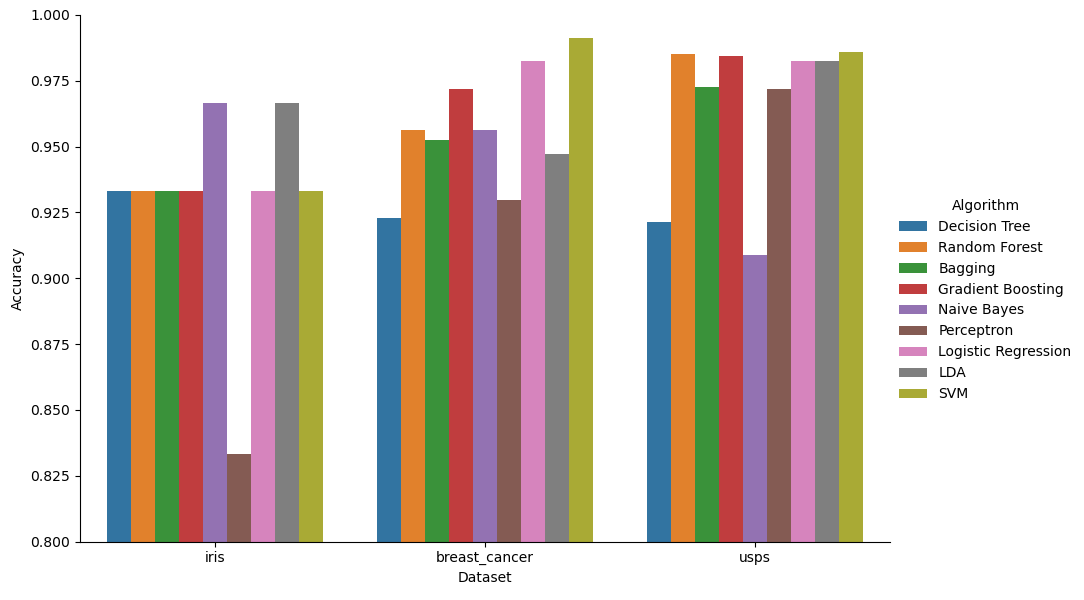
\includegraphics[width=12cm]{test.png}
  \caption{The accuracy on the test dataset for each model}
\end{figure}

\end{homeworkProblem}


% \newpage
% \Acknowledgement{Thank Siying Yang 2020012981 for
% the discussion about Problem 2.3 and Problem 3.}

% End edit to here
%%%%%%%%%%%%%%%%%%%%%%%%%%%%%%%%%%%%%%%%%%%%%%%%%%%%%%%%%%%%%

\end{spacing}
\end{document}

%%%%%%%%%%%%%%%%%%%%%%%%%%%%%%%%%%%%%%%%%%%%%%%%%%%%%%%%%%%%%
